\section{Erweiterung des Squarify Algorithmus} \label{sec:VerbesserungSquarify}
In diesem Abschnitt wird der Squarify Algorithmus \cite{bruls2000squarified}, wie er in Abschnitt \ref{sec:Squarify} beschrieben wurde, auf verschiedene Weisen erweitert und angepasst, um das Layoutproblem, wie es in Abschnitt \ref{sec:TreemapProblem} beschrieben wurde, anzugehen. 

\subsection{Approximative Fläche} \label{sec:ApproxFläche}
Die Grundlegende Idee dieser Erweiterung ist es, die Fläche der Knoten plus die Benötigte Fläche für die Abstände vor berechnung des Layouts zu approximieren.

Dafür brauche ich erstmal einen guten Algorithmus der das Layout gut macht, dann kann ich mit KI die Fläche lernen. Ist die frage ob das wirklich so gut funktionieren kann.

Problem man kann sich sehr gut beispiele konstuieren, bei denen das nicth funktionieren wird. Man kann das natürlich mit skalierung wieder lösen, aber das ist natürlich nicht optimal.

\subsection{Zweifache Berechnung} \label{sec:ZweifachBerechnung}

%HIER noch definieren die namen der schritte für bessere Lesbarkeit in den kapiteln danach z.b. layout schritt update schritt,...

Die Grundlegende Idee dieser Erweiterung ist es, dass sich die Fläche der Knoten mit Abstand durch das Layout und die Fläche der Knoten ohne Abstand approximieren lässt. Die Idee ist es also einen ersten Durchlauf zu machen, bei dem das Layout ohne Abstand berechnet wird. Dann werden die Größen der Knoten entsprechend dem Layout angepasst, sodass die Größe der Knoten nun auch den Abstand berücksichtigt. Anschließend wird ein zweiter Durchlauf mit diesen angepassten Größen durchgeführt, um das finale Layout zu berechnen.

Bevor wir uns die Details und Ergebnisse dieser Erweiterung anschauen, wollen wir vorweg nehmen, dass diese Erweitung natürlich nicht optimal funktionieren kann und das auch klar ist, da sich die die Änderung der Größe der Knoten natürlich auch das Layout im Zeweiten Durchlauf ändern wird, wodurch die Größen der Knoten wieder nicht korrekt sind. Was ja überhaupt erst das Grundlegende Problem ist (siehe Abshnictt \ref{sec:Problemstellung}). Allerdings ist es ein erster Schritt sich dem Problem zu nähern und zu schauen, ob es sich lohnt in diese Richtung weiter zu forschen.

Der Grundlegende Algorithmus bleibt also (fast) gleich, nur dass zwischen dem ersten und dem zweiten Durchlauf ein zusätzlicher Schritt \textit{Größenanpassung} eingefügt wird. Die Einzige änderung die vorgenommen werden muss ist, dass Knoten nur mit dem definierten Abstand zwischen dem Elternknoten platziert werden können und generell die Fläche des Elternknotens um den Abstand verkleinert wird.
Außerdem ist es nötig nach dem zweiten Durchlauf die Knoten, deren größenwert ja nun den abstand beinhalten, zu verkleinern, um auch den abstand zwischen den Geschwistern herzustellen. Es ist zu erkennen, dass dadurch der Abstand sowohl zwischen Geschwistern als auch zu den Elternknoten den doppelten wert des definierten Abstands hat, dieses Problem ignorieren wir hier, da man es trivialierweise lösen könnte, indem man immer nur die hälfte des Abstands zwischen Geschwistern und Elternknoten abzieht, was wir hier der einfachheit halber nicht tun. -- ODER VIELLEICHT HIER IN DER THESIS DOCH? DANN KÖNNTE ICH MIR DIESEN ABSCHNITT SPAREN, AUCH WENN ES IN DER IMPLEMENTIERUNG AM ENDE ANDERS IST

Wir stellen verschiedene Ansätze vor, was sowohl die Größenanpassung als auch die Anpassung der Knoten nach dem zweiten Durchlauf angeht.
Die Algorithmen funktionieren allerdings alle nach ähnlichem Prinzip: Es wird zunächst für jeden Knoten die Fläche die der Abstand in diesem Layout benötigen würde addiert, indem die Fläche aus der neuen Länge (alte Länge + 2 mal den Abstand) und der neuen Breite (alte Breite + 2 mal den Abstand) berechnet wird. Zusätzlich wird für Elternknoten die Flächenvergrößerung aller Kindernkoten addiert. An dieser Stelle ist allerdings nicht klar, wie sich die Flächenvergrößerung der Kinderknoten auf die Fläche der Elternknoten auswirkt, da diese Änderung selbst von der Anordnung der Kinderknoten abhängt. Wir testen verschiedene Ansätze, um die Flächenänderung der Elternknoten in Abhängikeit zu der Flächenänderung der Kinderknoten zu approximieren.

Nach dem zweiten Durchlauf wird nun die Fläche der Knoten so reduziert, dass sowohl der Abstand zwischen Geschwistern als auch der Abstand zu den Elternknoten den gewünschten Wert hat. Dies ist straight forward und wird hier nicht weiter erläutert. Anzumerken ist aber das dieser Schritt speziell abhängt von der Art der Größenanpassung, die im ersten Schritt durchgeführt wurde.

\subsubsection{Einfache Größenanpassung}
Dies ist die einfachste naive Version der Größenanpassung, der Algorithmus zeigt aber gut die zuvor beschriebenen Probleme auf. Die Fläche der Knoten wird um den Abstand in beiden Richtungen vergrößert. Zusätzlich wird die Fläche der Elternknoten um die Fläche der Kinderknoten vergrößert. 

\begin{algorithm}[H]
\caption{Einfache Größenanpassung}
\label{alg:EinfacheGrößenanpassung}
\begin{algorithmic}[1]
\Function{increaseValuesSimple}{node: SquarifyNode, margin: number}
    \State childrenValueIncrease $\gets$ 0
    \If{node.children}
        \For{child in node.children}
            \State childrenValueIncrease += increaseValuesSimple(child, margin)
        \EndFor
    \EndIf
    \State valueIncrease $\gets$ width * margin * 2 + length * margin * 2 + margin * margin * 4 + childrenValueIncrease
    \State node.value += valueIncrease
    \State \Return valueIncrease
\EndFunction
\end{algorithmic}
\end{algorithm}

Das Problem des Algorithmuses ist am besten an einem Beispiel zu verdeutlichen. Wir visualieren den ZWITEN AnHANG - auch wieder eine händisch erstellte Map, um das Problem zu verdeutlichen. In Abbildung \ref{fig:zeroMarginSquarifyArtifialTwo} ist das Layout mit einem Abstand von 0 zu sehen. 

\begin{figure}
    \centering
    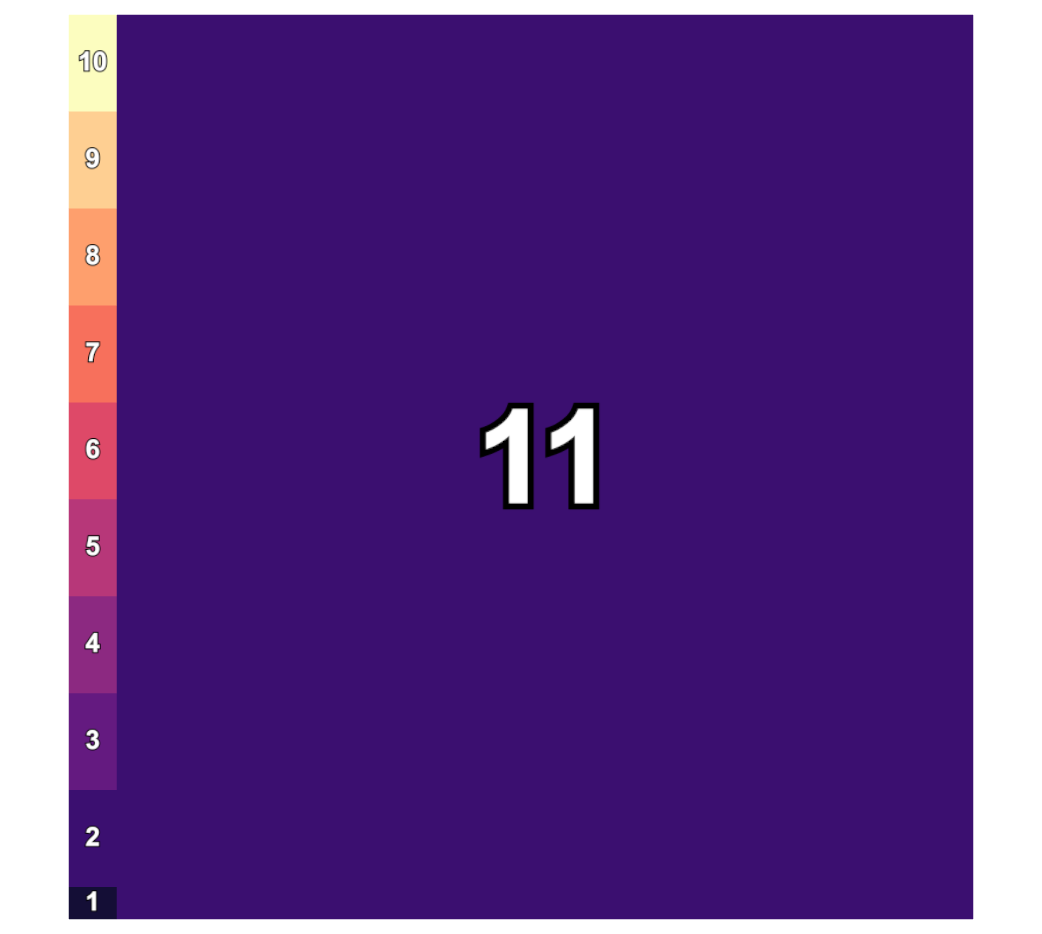
\includegraphics[width=0.8\textwidth]{images/zeroMarginSquarifyArtifialTwo.png}
    \caption{Treemap Layout generiert mit dem Squarify Algorithmus nach Abschnitt \ref{sec:Squarify} mit einem Abstand von 0 und der einfachen Größenanpassung auf der händisch erstellen map (siehe Anhang).}
    \label{fig:zeroMarginSquarifyArtifialTwo}
\end{figure}

In Abbildung \ref{fig:simpleIncreaseMarginOne} ist das Layout mit einem Abstand von 1 zu sehen. Es ist zu erkennen, dass die Knoten auf der linken Seite des Layouts sich außerhalb ihrer Elternknoten erstrecken. Warum passiert das? Knoten 10 ist im zweiten Layout-Schritt deutlich schmaler als im ersten Layout-Schritt. Dadurch wird die Fläche die durch den Abstand eingenommen wird größer als angenommen, weshalb die Fläche des Knotens nach abzug des Abstands im letzen Schritt kleiner ist, als gewünscht. Dementsprechend ist auch die Fläche der Knoten unten links größer als gewünscht, da das Layout der Knoten im zweiten Layout-Schritt quadratischer wird. Knoten 5, der Knoten, der am Quadratischsten ist, wird also am größten erscheinen. Obwohl beide den selben wert haben ist Knoten 5 ca. 1,2 mal größer als Knoten 10) In diesem Beispiel erscheint der unterschied kaum merklich, aber es gibt ihn trotzdem und in anderen fällen kann dieser Unterschied merklich werden.
Viel signifikanter ist aber der Effekt, dass Elternknoten ebenfalls immer schmaler werden, wodurch die fläche, die der innerere abstand einnimm, ebenfalls größer wird und dass sogar immer mehr von ebene zu ebene, wenn man runter geht. Dadurch wird die Fläche für die Kindknoten immer kleiner, was dazu führt, dass Knoten teilweise über ihre Elternknoten hinauswachsen.

\begin{figure}
    \centering
    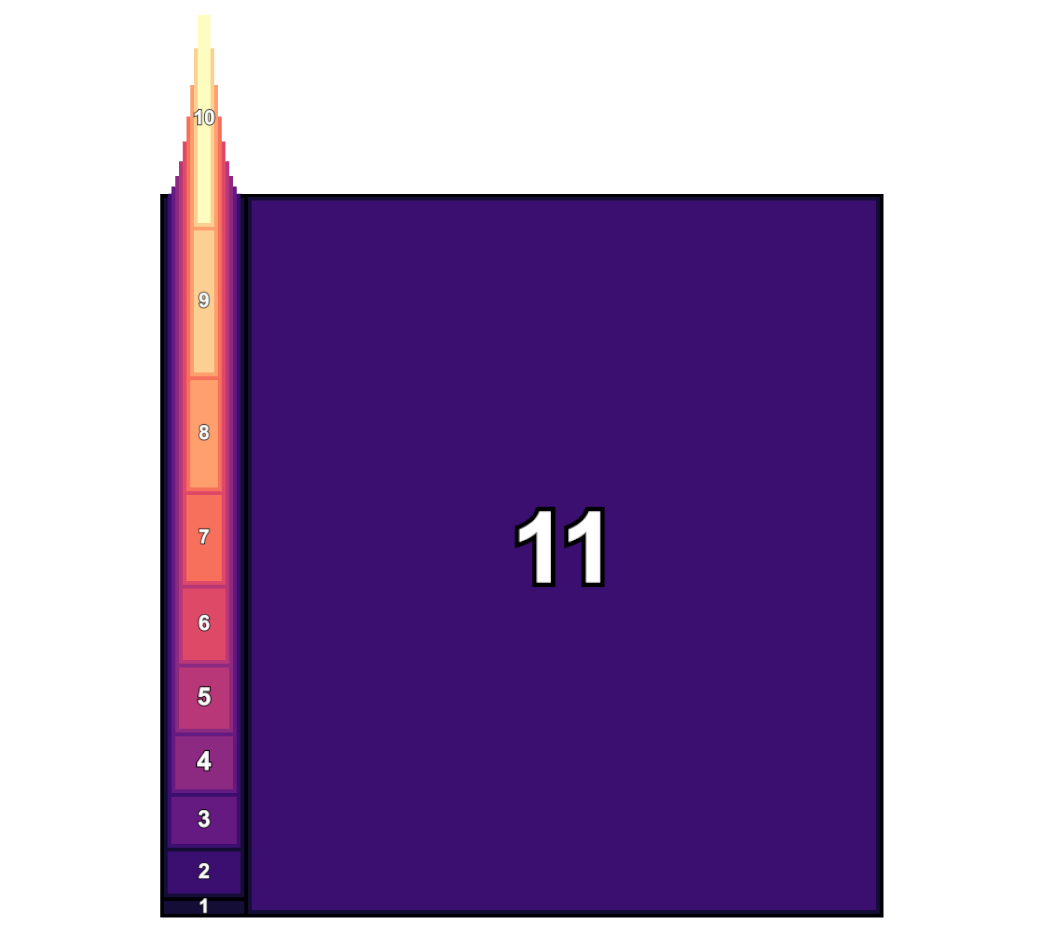
\includegraphics[width=0.8\textwidth]{images/simpleIncreaseMarginOne.png}
    \caption{Treemap Layout generiert mit dem Squarify Algorithmus nach Abschnitt \ref{sec:Squarify} mit einem Abstand von 1 und der einfachen Größenanpassung auf der händisch erstellen map (siehe Anhang).}
    \label{fig:simpleIncreaseMarginOne}
\end{figure}

Dieser Effekt kann einfach behoben werden, wie wir in Abschnitt \ref{sec:ScalingKnoten} sehen werden.

\subsubsection{Relative Größenanpassung}
Bei der berechnung zuvor wurde einfach der margin fläche eines Elternknotens berechnet, auf basis der alten Fläche, ohne die Flächenädnerung durch die Kinderknoten zu berücksichtigen. dadurch wird die resultierende Fläche der Elternknoten zu klein sein, da die Fläche der Kinderknoten nicht berücksichtigt wird.
Die Idee bei dieser Erweiterung ist es die Änderung der Kinder schon vor dem Hinzufügen der Abstandsfläche zu berücksichtigen. Dafür muss die relative Flächenänderung durch die Kindknoten berechnet werden. und damit dann die Seitenlängen anpassen und dann die margins hinzufügen, um die neue Fläche zu erhalten.
Der Algorthmus wird im foldenden als Pseudocode dargestellt (siehe Algorithmus \ref{alg:ZweifachBerechnung}). 

\begin{algorithm}[H]
\caption{Relative Größenanpassung}
\label{alg:ZweifachBerechnung}
\begin{algorithmic}[1]
\Function{increaseValues}{node: SquarifyNode, margin: number}
    \State childrenValueIncrease $\gets$ 0
    \If{node.children}
        \For{child in node.children}
            \State childrenValueIncrease += increaseValues(child, margin)
        \EndFor
    \EndIf

    \State ratioChildrenValueIncrease $\gets$ (node.value + childrenValueIncrease) / node.value

    \State valueIncrease $\gets$ 
        Math.sqrt(ratioChildrenValueIncrease) * width * margin * 2 +
        Math.sqrt(ratioChildrenValueIncrease) * length * margin * 2 +
        margin * margin * 4 +
        childrenValueIncrease

    \State node.value += valueIncrease
    \State \Return valueIncrease
\EndFunction
\end{algorithmic}
\end{algorithm}

Problem:
Der Algorithmus in dieser Form zeigt einige Probleme auf. Die Flächenvergrößerung der Kindknoten sagt nichts darüber aus, in welche Richtung sich die Fläche ändert. Es wird davon ausgegangen, dass sich die Fläche gleichmäßig in beide Richtungen ändert (siehe Zeile 13 und 14 in Algorithmus ZEILEN ANPASSEN  \ref{alg:ZweifachBerechnung}). 
es kommt also zu ähnlichen Problem wie davor. es können knoten sowohl zu viel platz als auch zu wenig Platz bekommen, jenachdem ob Sie im zweiten schritt quadratischer oder schmaler werden.  Siehe Abbildung \ref{fig:relativeIncreaseMarginOne} für ein Beispiel.

\begin{figure}
    \centering
    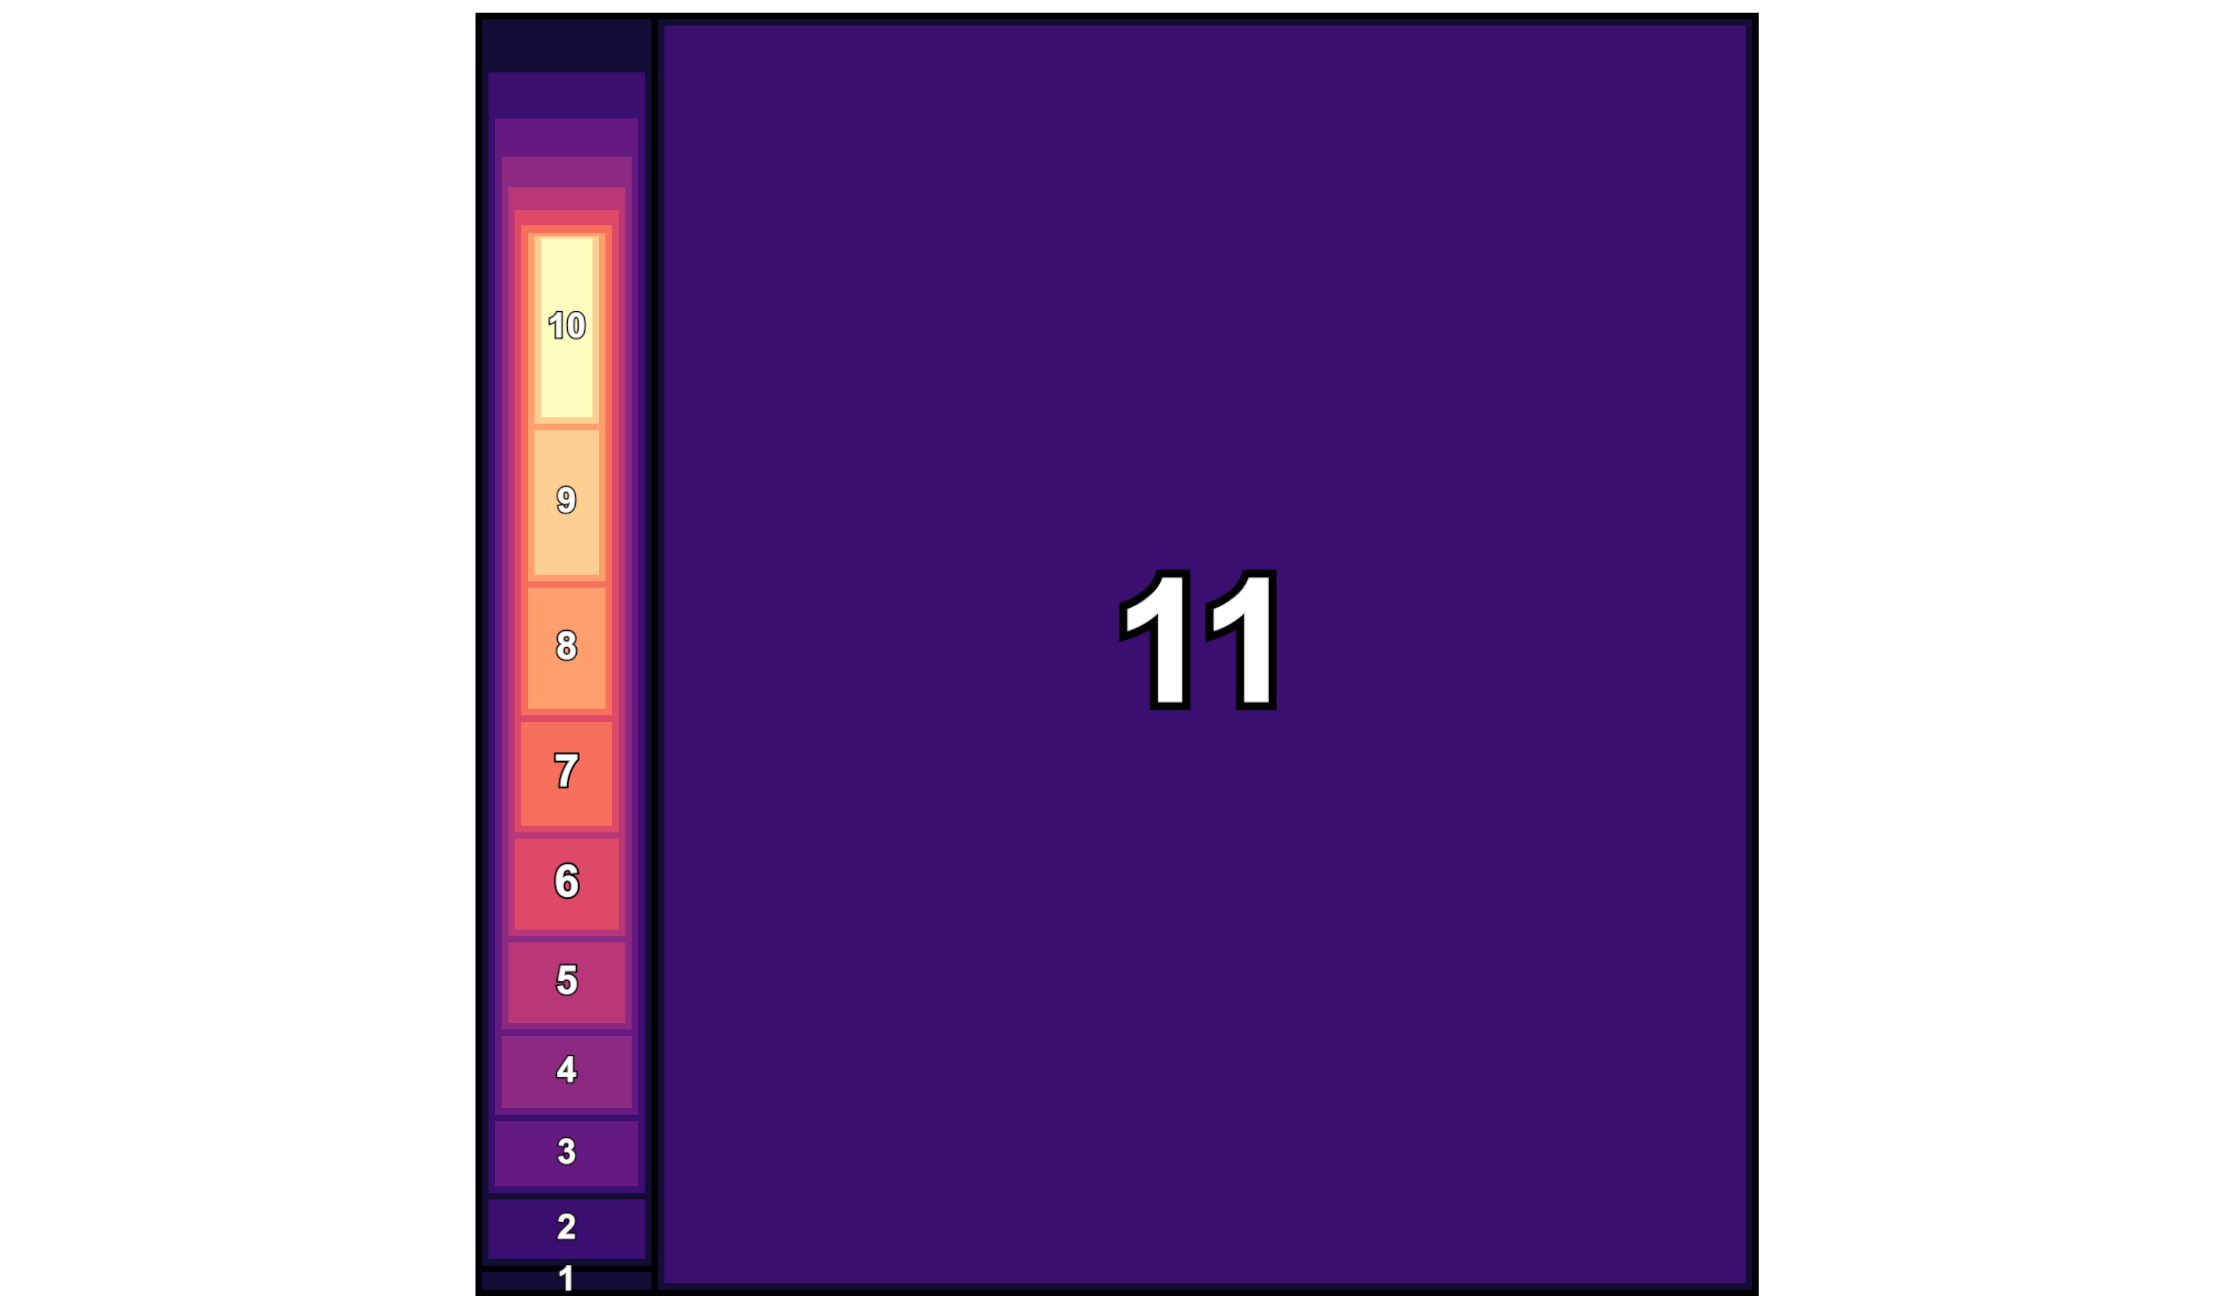
\includegraphics[width=0.8\textwidth]{images/increaseMarginOne.png}
    \caption{Treemap Layout generiert mit dem Squarify Algorithmus nach Abschnitt \ref{sec:Squarify} mit einem Abstand von 1 und der relativen Größenanpassung auf der händisch erstellen map (siehe Anhang).}
    \label{fig:relativeIncreaseMarginOne}
\end{figure}

\subsection{Scaling der Knoten} \label{sec:ScalingKnoten}
Wenn die Fläche innnerhalb von Elternknoten immer kleiner wird, kann es passieren, dass Knoten über ihre Elternknoten hinauswachsen, wie in Abbildung \ref{fig:simpleIncreaseMarginOne} zu sehen ist. Es kann genauso passieren, dass die Fläche innerhalb der Knoten größer wird, wie in Abbildung \ref{fig:relativeIncreaseMarginOne} auf der linken seite zu erkennen ist. Dieser Effekt kann trivialer weise behoben werden, indem der zweite Layout-Schritt angepasst wird, sodass die Knoten immer auf die Fläche des Elternknotens skaliert werden. 
Vor jeden Squarify-Schritt wird dafür die wirklich zur verfügung stehende Fläche des Elternknotens berechnet und die Kindknoten entsprechend dieser Änderung skaliert, sodass sie genau in die Fläche des Elternknotens passen.

Der Nachteil dieser Methode ist in Abbildung \ref{fig:simpleIncreaseMarginOneScale} zu erkennen. Die Knoten werden dadurch natürlich nicht mehr proportional zu ihren Werten sein. Knoten 10 hat zum beispiel ein Verhältnis von ca. 0.5 zu seinem Wert, während Knoten 6 ein Verhältnis von ca. 1.4 zu seinem Wert hat.

\begin{figure}
    \centering
    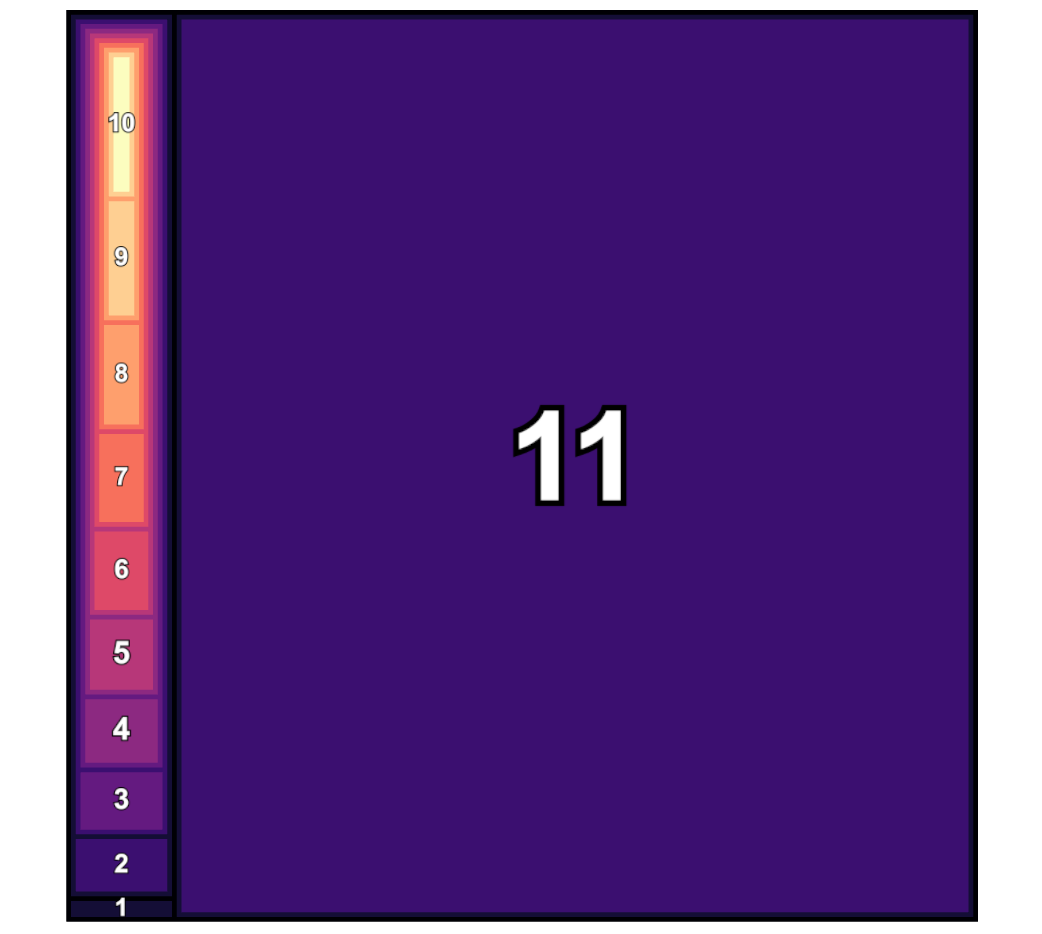
\includegraphics[width=0.8\textwidth]{images/simpleIncreaseMarginOneScale.png}
    \caption{Treemap Layout generiert mit dem Squarify Algorithmus nach Abschnitt \ref{sec:Squarify} mit einem Abstand von 1 und der einfachen Größenanpassung auf der händisch erstellen map (siehe Anhang) und der Skalierung der Knoten.}
    \label{fig:simpleIncreaseMarginOneScale}
\end{figure}

Je genauer die Größenanpassung der Knoten ist, desto geringer fällt natürlich dieser Effekt aus. Siehe im Vergleich dazu Abbildung \ref{fig:relativeIncreaseMarginOneScale}, da die relative Größenanpassung deutlich genauer ist, ist der Effekt hier auch deutlich geringer. Knoten 10 hat Größe 40 und Knoten 6 hat Größe 41, was fast ähnlich Groß ist.

\begin{figure}
    \centering
    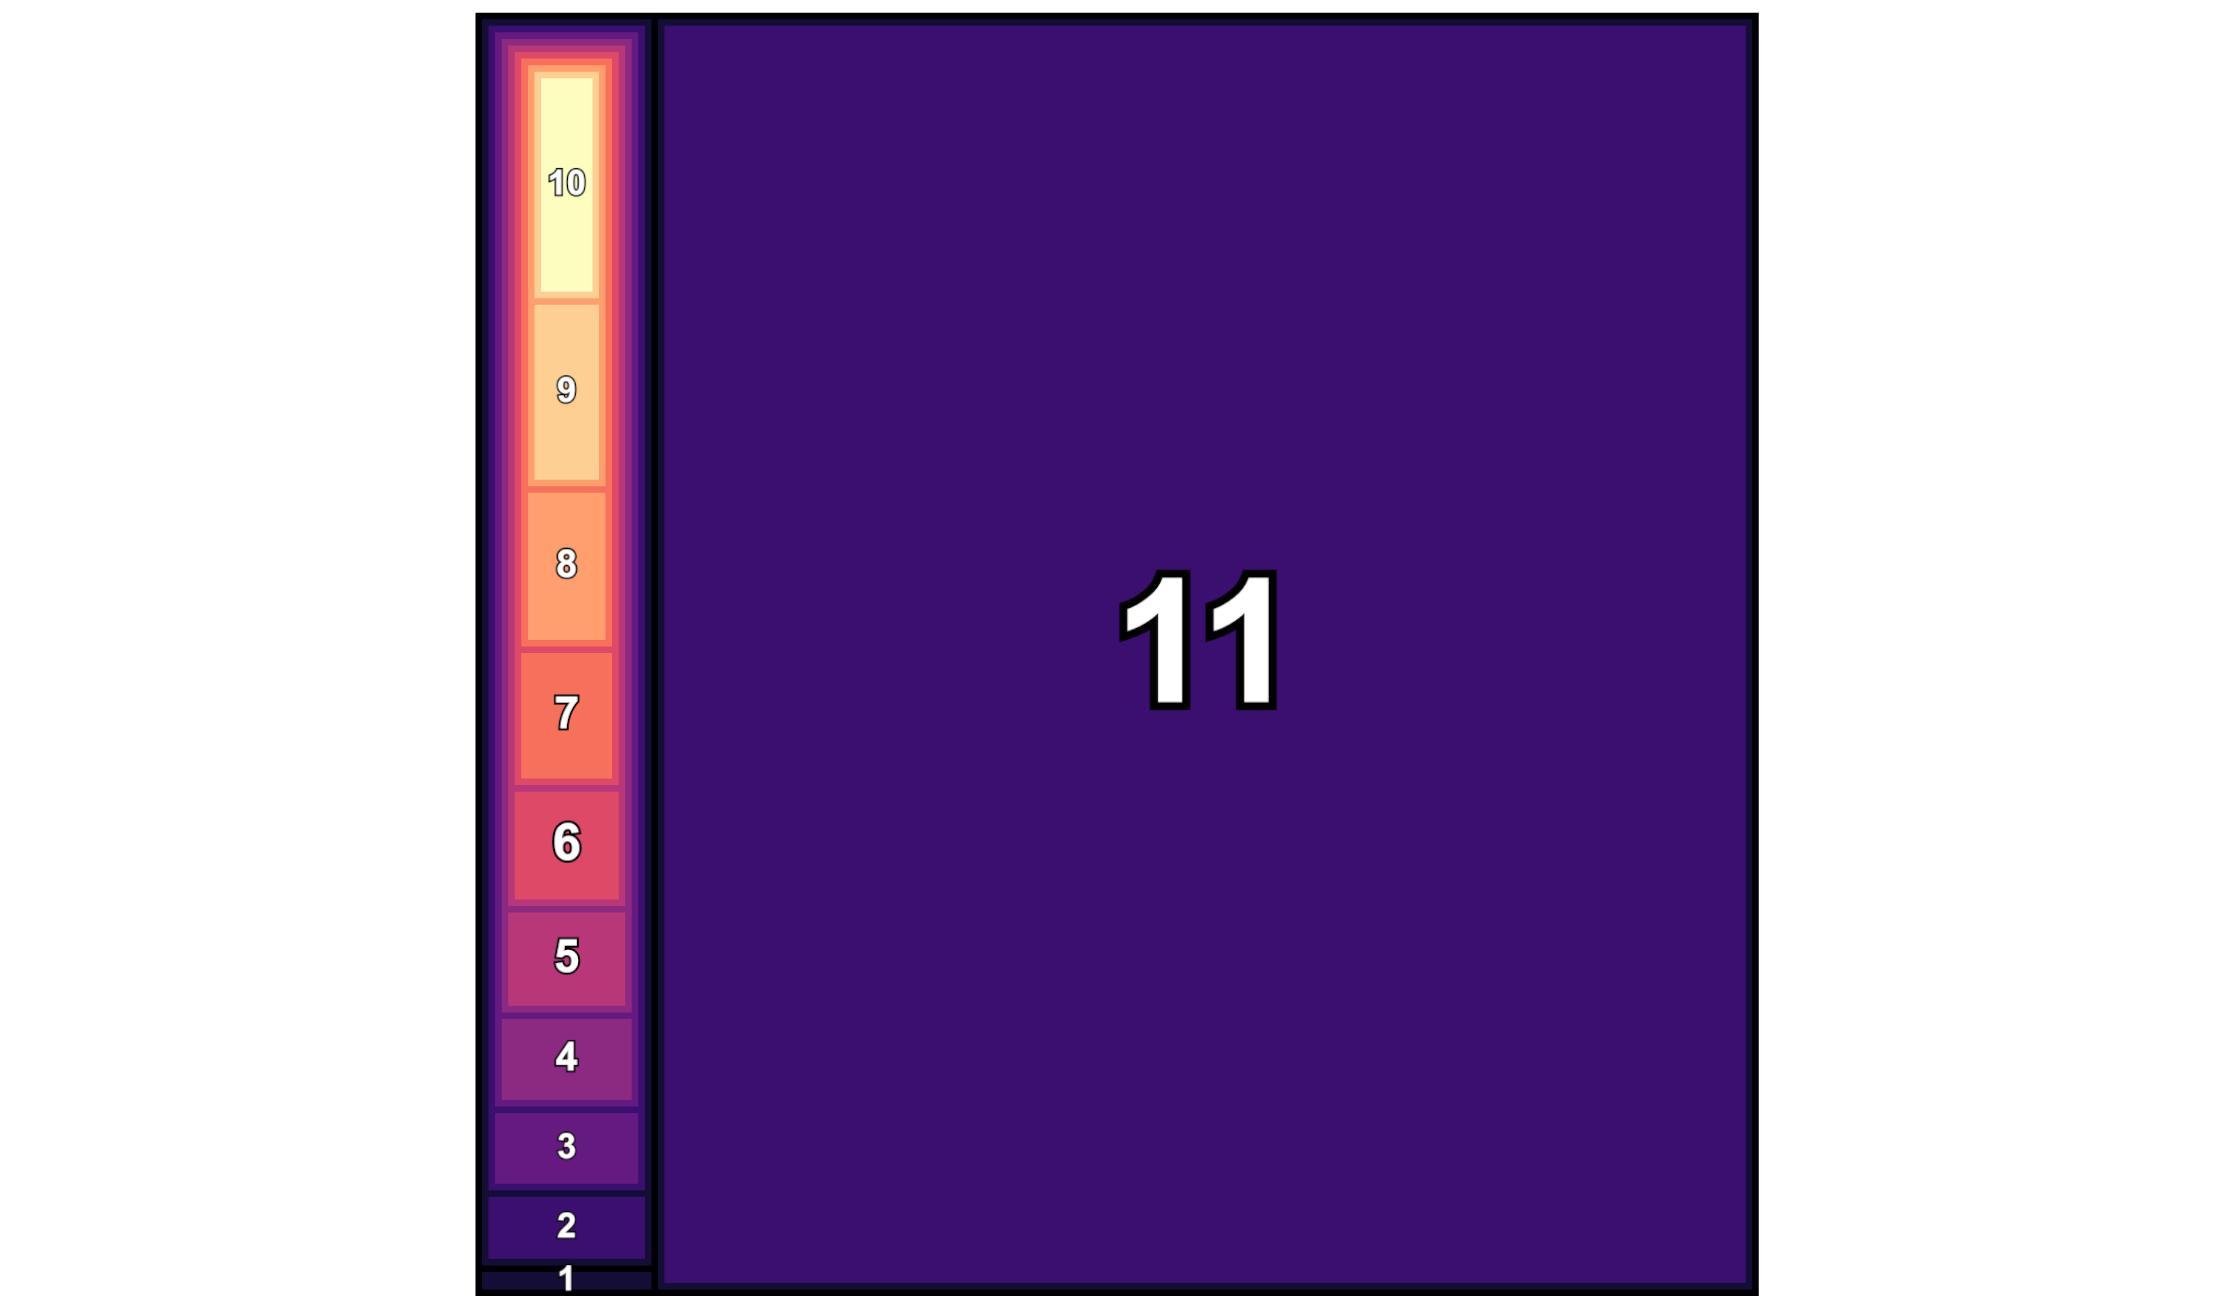
\includegraphics[width=0.8\textwidth]{images/increaseMarginOneScale.png}
    \caption{Treemap Layout generiert mit dem Squarify Algorithmus nach Abschnitt \ref{sec:Squarify} mit einem Abstand von 1 und der relativen Größenanpassung auf der händisch erstellen map (siehe Anhang) und der Skalierung der Knoten.}
    \label{fig:relativeIncreaseMarginOneScale}
\end{figure}

Persönlich würde ich sagen, dass dieser Effekt für das herunter skalieren der Knoten gut ist, da sonst eine grundlegende eigenschaft der Darstellung verletzt wird, aber für das hoch skalieren der Knoten könnte man auch sagen, dass es wichtiger ist die Fläche der Knoten proportional zu ihren Werten zu halten, als die \textit{verschwendete} Fläche aufzufüllen. Diese jetzt hier sehr subjektive Einschätzung wird aber nochmal genauer beläuchtet in der evaluation und vergleich.

\subsection{Reihenfolge der Knoten im ersten Layoutschritt} \label{sec:ReihenfolgeKnoten}
Die Reienfolge in der die knoten in das Layout eingefügt werden, hat einen großen Einfluss auf das Layout. \cite{johnson1991tree} haben in ihrem Paper herausgefunden, dass die ergebnisse am besten sind, wenn die Knoten in der Reihenfolge der Größe eingefügt werden. Also der Größte zuerst.
%was machen wir damit?

\subsubsection{Reihenfolge der Knoten nach erstem Layoutschritt} \label{sec:ReihenfolgeKnotenErstesLayout}
Durch die updates der Größen der Knoten nach dem ersten Layoutschritt, kann es passieren, dass die Größenreihenfolge der Knoten sich ändert. Das als zum Beispiel Knoten A im ersten Layoutschritt größer ist als Knoten B, aber nach dem Update der Größen von Knoten A kleiner ist als Knoten B. Das kann dazu führen, dass im folgenden Layoutschritt, die Knoten in einer anderen Reihenfolge platziert werden als im ersten Layoutschritt. 
Das ist erstmal gut für die Seitenverhältnisse der Knoten (wenn wir davon ausgehen, dass die Reihenfolge nach größe sortiert optimla ist), allerdings kann es dazu führen, dass Knoten an ganz anderen Positionen platziert werden, als im ersten layoutschritt. Das  kann dazu führen, dass sich die Form ändert und das kann dazu führen, dass die Kinder anders platziert werden etc. wodurch sich die benötigten Abstände ändern, wodurch die vorausberechnete Fläche der Knoten nicht mehr passt und Knoten entweder verschwinden oder die Wert Fläche relation schlechter wird.
Das kann natürlich genauso passieren, wenn die Knoten in der selben Reihenfolge platziert werden, wie im ersten Layoutschritt. Es ist nicht klar erstichtlich, was hier am Ende des Tagen am besten ist. Deswegen implementieren wir 3 verschiedene Ansätze:
\begin{itemize}
    \item \textbf{Reihenfolge der Knoten nach Größe:} Die Knoten werden in der Reihenfolge ihrer Größe platziert. Wir vermuten, dass dadurch die besten Seitenverhältnisse entstehen, aber die schlechtesten WErt-Fläche-Relationen.
    \item \textbf{Reihenfolge der Knoten beibehalten:} Die Knoten werden in der Reihenfolge platziert, in der sie im ersten Layoutschritt platziert wurden. Wir vermuten, dass dadurch im Großen und Ganzen die plazierung der Knoten gleich bleibt, außer es gibt wirklich große Flächen updates. Wir vermuten, dass dies ein guter mitelweg zwischen dem ersten und dem jetzt folgenden ansatz ist.
    \item \textbf{Platzierung der Knoten beibehalten:} Nach dem ersten Layoutschritt wird sich genau die Aufteilung der Knoten in Reihen und die Platzierung der Knoten in den Reihen gemerkt. Wir vermuten, dass dadurch die Form der Knoten im großen und ganzen ähnlich zum ersten Schritt bleibt, wodurch die Wert-Fläche-Relationen besser bleibt, aber die Seitenverhältnisse schlechter werden könnten, die die optimale Reihenfolge der Knoten (aufgrund der neuen werte) nicht mehr berücksichtigt wird.
    \item 
\end{itemize} 
Es ist wie gesagt nicht ganz klar, was genau die auswirkungen sind. deswegen nur vermutungen, die wir jetzt testen werden.

%wie häufig passiert das?
%wie sehr ändert sich die reiehenfolge der Knoten?
%Wie sehr ändert sich die position der Knoten?
%sind das überhaupt relevante Fragen? - oder ist nur wichtig das Seitenverhältnis und Wert-Fläche-Relationen gut sind?

\subsection{Mehrfache Berechnung} \label{sec:MehrfacheBerechnung}
Die Grundlegende Idee dieser Erweiterung ist es, das Layout mehrfach zu berechnen und dabei die Fläche der Knoten immer weiter anzupassen. 
Warum glauben wir, dass das gut ist. nach dem ersten update schritt ist die vorhersage der neuen fläche ja oft nicht so gut, und es kann sich noch einiges in der reihenfolge der Knoten ändern oder die Form der Knoten. dadurch ist nach dem zweiten Layout-Schritt die platzierung ja anders, dadurch stimmt die vorhergesagte Fläche der Knoten nicht mehr. dann könnte man nochmal her gehene und die fläche neu berechnen und nochmal den layoutschritt machen. 

Grund dafür:
Grund dagegen: 

\subsubsection{Iterative Abstandsvergrößerung} \label{sec:IterativeAbstandsvergrößerung}
In bild updateValues.png ist zu erkennen, dass kp. margin 10 noP 3

Die Grundlegende Idee dieser Erweiterung ist es, das wenn das Layout mehrfach berechnet wird, es besser ist, den Abstand zwischen den Knoten iterativ von Schritt zu Schritt zu vergrößern, anstatt ihn von Anfang an auf den finalen Wert fest zu setzen. 
Warum gehen wir von dieser Annahme aus? 
Wenn man im ersten Schritt den Abstand auf den finalen Wert setzt, dann werden die Vorhersagen für die neue Fläche der Knoten im zweiten Schritt nicht exakt sein, das ist ja klar. Umso kleiner die Abstände sind, umso kleiner sind auch die Abweichungen dieser Vorhersagen. Dadurch sollten die Wer-Fläche-Relationen im zweiten Schritt besser sein. 
%zeige das anhand von daten
Die Annahme ist jetzt, dass wenn man jedes mal den Abstand um einen kleinen Wert vergrößert, dann sind in jedem Schritt die Vorhersagen für die Fläche der Knoten genauer, wodurch die Wert-Fläche-Relationen besser werden. Als Gegenargument könnte man bringen, dass dadurch, dass jedes mal die Abstände größer werden auch jedes mal das Optimale Layout (man kann das optimale layout nicht berechnen, aber wir gehen mal von einem theoreitschen optimalen Layout aus) auch in jedem layout schritt anders sein wird. Dadurch wird erst im letzen Layoutschritt das "wahre" optimale Layout angestrebt, wodurch die vorherigen schritte unnötig waren.

Wir überprufen jetzt die annahme und schauen, welche begründung richtiger ist/welcher effekt mehr gewicht hat. 
hier ist es auch interessant den effekt in kombination mit der Reihenfolge der Knoten zu testen, weil %warum eigentlich?

\subsection{Änderungen im Layout} \label{sec:LayoutÄnderungen}
Folgend werden Änderungen beschrieben, die sich sichtbar auf die Visualierung auswirken und nicht nur auf Platzierung, Größe, Form,... etc der Knoten. Diese Änderungen zielen trotzdem vorallem darauf ab, das Treemap-Layout-Problem zu lösen bzw. abzuschwächen, machen dies aber vorallem durch visuelle Anpassungen und nicht durch komplexe algorithmische Anpassungen.

\subsubsection{Optimierung von Ordnerketten} \label{sec:OrderKetten}
Bei der Datenanalyse ist aufgefallen, dass es oft vorkommt, dass Ordner nur ein Kind haben bzw. dass es \textit{Ketten} von Ordnern gibt, die nur ein Ordner als Kind haben. Diese Struktur wird zum Beispiel für Module in Java/Kotlin verwendet.
Zum Beispiel im OpenSource Projekt CodeCharta 
codecharta/analysis/analysers/AnalyserInterface/src/main/kotlin/de/maibornwolff/codecharta/analysers/analyserinterface/AnalyserInterface.kt
Ab dem Ordern \textit{main} bis zum Ordner \textit{analyserinterface} geht die Kette von Ordnern.
Durch diese tiefe Verschachtelung wird viel Platz für die Abstände zwischen den Ordnern verbraucht, obwohl im Grunde diese Schachtelung keine wirklichen Strukturinformationen enthält. Viele IDEs wie zum Beispiel auch IntelliJ IDEA oder VSCode verbergen diese Ordnerstruktur zum beispiel auch automatisch, in dem solche ordner ketten nur als ein Ordner mit entsprechendem zusammen gefügten namen (in dem fall \textit{main/kotlin/de/maibornwolff/codecharta/analysers/analyserinterface}) angezeigt wird.
Diese Optimierung kann auch für unsere Visualisierung übernommen werden, indem solche Ordnerketten zu einem Ordner zusammengefasst werden. 
Es ergeben sich folgende Auswirkungen auf die Ziele der Visualisierung:
\begin{itemize}
\item \textbf{Informationsgehalt und effiziente Nutzung des Platzes:} Wird verbessert, da weniger Platz für Abstände zwischen den Ordnern benötigt wird und weniger Knoten im Layout sind. 
    \item \textbf{Niedrige visuelle Komplexität und hohe Verständlichkeit:} Wird verbessert, da weniger Knoten im Layout sind und tiefe Verschachtelungen vermieden werden.
    \item \textbf{Skalierbarkeit:} Wird verbessert, da weniger Knoten im Layout sind und die Berechnung des Layouts beschleunigt wird.
    \item \textbf{Korrelation mit dem Code:} wird verschlechtert, da die Ordnerstruktur nicht mehr 1:1 mit der Code-Struktur übereinstimmt. die \textit{wahre} Tiefe der Ordnerstruktur nicht mehr ersichtlich ist. Allerdings ist die Tiefe der Ordnerstruktur selbst in eigentlich gar nicht so relevant, die Tiefe wird eher als Mittel benutzt um die Ordner Struktur darzustellen. Ob eine Datei jetzt 5 oder 10 tief liegt, macht für die WAhrnehmung der Struktur keinen großen Unterschied.
    \item \textbf{Stabilität gegenüber Änderungen:} Wird verbessert, da durch weniger Abstände die differenz zwischen Knoten Fläche und Knoten Wert geringer werden, wodurch weniger umstrukturierung bei der Platzierung der Knoten nötig ist. Außerdem wirken sich trivialerweise Änderungen an Order-Ketten nicht mehr auf die gesamte Struktur aus und verändern somit auch die Visualierung nicht, was positiv für die stabilität ist (aber wie gesagt negativ für die Korrelation mit dem Code).
\end{itemize}
Wir würden sagen, dass die Vorteile dieser Änderung die Nachteile stark überwiegen.

Im Schnitt werden ca. 175 Ordner pro Codebasis gefaltet (12 Median). bei ca. 958 Knoten (Median 242) sind das ca. 18\% (bzw. 5\% Median) der Knoten die durch die Faltung verschwinden. Also schon einige. 

Folgend kommen die DAten:

\begin{figure}
    \centering
    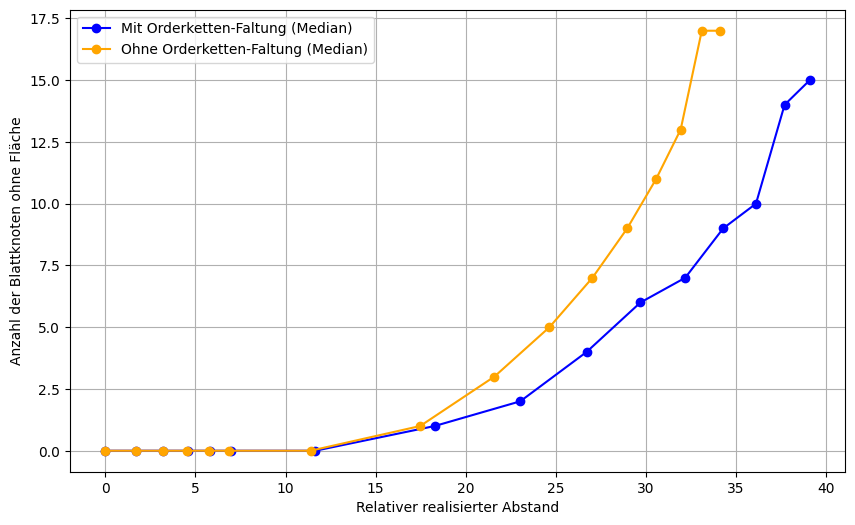
\includegraphics[width=0.8\textwidth]{images/improve/FaltungBlattknotenOhneFlaeche.png}
    \caption{Die Anzahl der Knoten ohne Fläche geplottet gegenüber des Abstandes. Es ist zu erkennen, dass das Falten von Ordnerketten die das verschwinden von Knoten reduziert.}
    \label{fig:FaltungKnotenOhneFlaeche}
\end{figure}

\begin{figure}
    \centering
    \includegraphics[width=0.8\textwidth]{images/improve/FaltungWertFlaecheVerhältnis.png}
    \caption{Das Wert-Fläche-Verhältnis der Knoten geplottet gegenüber des Abstandes. Es ist zu erkennen, dass das Falten von Ordnerketten das Wert-Fläche-Verhältnis der Knoten verbessert.}
    \label{fig:FaltungWertFlaecheVerhältnis}
\end{figure}

\begin{figure}
    \centering
    \includegraphics[width=0.8\textwidth]{images/improve/FaltungSeitenverhältnis.png}
    \caption{Das Seitenverhältnis der Knoten geplottet gegenüber des Abstandes. Es ist nicht klar zu erkennen, ob das Falten von Ordnerketten das Seitenverhältnis der Knoten verbessert oder verschlechtert, deshalb sind die Bereiche des Positiven effekts grün markiert und die Bereiche des negativen Effekts rot markiert. Es zeigt sich ein leicht positiver Effekt besonders bei kleinen und großen Abständen.} 
    \label{fig:FaltungSeitenverhältnis}
\end{figure}

\begin{figure}
    \centering
    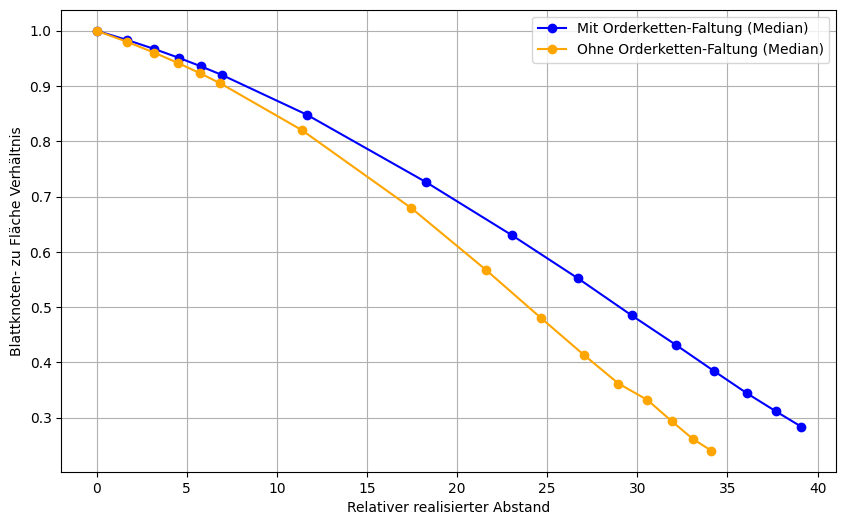
\includegraphics[width=0.8\textwidth]{images/improve/FaltungBlattFlaeche.png}
    \caption{Die Fläche der Blattknoten in Verhältnis zu der gesamt Fläche geplottet gegenüber des Abstandes. Es ist zu erkennen, dass das Falten von Ordnerketten die Fläche der Blattknoten erhöht. Das heißt, es wird weniger Platz benötigt für Abstände und Ordner, also gleiche Informationen auf weniger Fläche, beduetet besserer Informationsgehalt.}
    \label{fig:FaltungBlattFlaeche}
\end{figure}

\begin{figure}
    \centering
    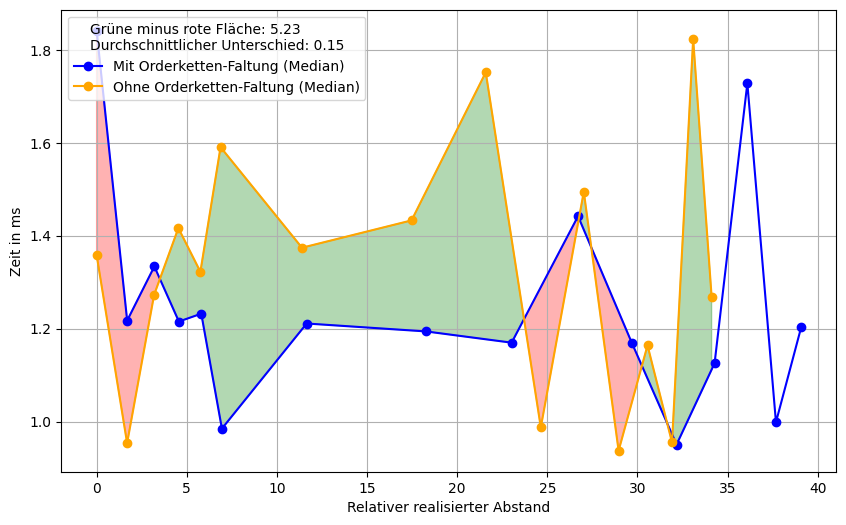
\includegraphics[width=0.8\textwidth]{images/improve/FaltungZeit.png}
    \caption{Die Rechenzeit geplottet gegenüber des Abstandes. Es ist nicht klar zu erkennen, ob das Falten von Ordnerketten die Rechenzeit verbessert oder verschlechtert, deshalb sind die Bereiche des Positiven Effekts grün markiert und die Bereiche des negativen Effekts rot markiert. Die Schwankungen sind zwischen ungefähr 1 und 2 millisekunden, was nicht wikrlich ausschlaggebend ist. Trotzdem ist ein leichter perfomance gewinn zu erkennen beim falten, was wahrscheinlich einfach daran liegt, dass es weniger Knoten gibt.}
    \label{fig:FaltungZeit}
\end{figure}

die Daten Zeigen in allen Aspekten eine Verbesserung durch das Falten von Ordnerketten. Wir sprechen uns also dafür aus, dass Ordnerketten immer gefaltet werden sollten, von den messbaren Kriterien her sehen wir keine Gründe, warum das nicht gemacht werden sollte. das einzige Ziel was dagegen spricht ist die Korrelation mit dem Code, die dadurch verschlechtert wird. Alles in allem sprechen wir uns also dafür aus und werden dies fix für unseren Algorithmus implementieren.

\subsubsection{Beschriftung der Knoten} \label{sec:BeschriftungKnoten}
Die Beschriftung der Knoten ist ein wichtiger Aspekt der Visualisierung, da sie es dem Nutzer ermöglicht, die Knoten zu identifizieren und zu verstehen, welche Informationen sie repräsentieren. Es gibt verschiedene Ansätze, um die Beschriftung der Knoten zu gestalten. Jeder Ansatz hat seine Vor- und Nachteile. Ein häufig verwendeter Ansatz ist wie zum Beispiel auch beim in Abschmijt VerwandteArbeiten \ref{sec:VerwandteArbeiten} vorgestellten Cascaded Treemap Ansatz \cite{lu2008cascaded}.
Ordner erhalten eine Zusätzliche horizontale Fläche, entweder unten oder oben, die den Namen des Ordners enthält. 
Dies nimmt allerdings viel Platz ein und erzeugt die selben schwierigkeiten für den Algorithmus, wie die abstände zwischen den Knoten. Außerdem kann es passieren, dass die Beschriftung zu lang für die breite der Knotens ist, wodurch die Beschriftung entweder abgeschnitten wird oder über den Knoten hinauswächst.
Hao Lü and James Fogarty schlagen vor dynamisch zu entscheiden, ob die Beschriftung der Knoten angezeigt werden soll oder nicht \cite{lu2008cascaded}. Wenn das Hinzufügen der Beschriftung den Knoten dazu führen würde, dass gar kein Platz mehr für den Knoten selbst übrig bleibt, wird die Beschriftung nicht angezeigt. Der Vorteil dieses Ansatzes ist, dass sicher gegangen wird, dass durch die Beschriftung kein Knoten verschwindet. Der Nachteil ist, dass selbst wenn die Änderung der Knotenfläche zum Knotenwert durch das hinzufügen der Beschriftung riesig wird (wenn die Fläche also super klein wird), die Beschriftung trotzdem hinzugefügt wird. 

Wir schlagen einen statischen ansatz vor, bei dem nur die Beschriftungen der Top N order angezeigt werden. 
Die Wahl von N ist nun die Stellschraube für die nicht für jede Codebasis gleich ist. Es ist Stellschraube um zwischen Informationsgehalt und visuelle Komplexität zu balancieren.
\begin{itemize}
    \item Je höher N ist, desto mehr Informationen (also Ordnernamen) werden angezeigt, was den Informationsgehalt erhöht.
\item Je niedriger N ist, desto weniger Informationen werden angezeigt, was die visuelle Komplexität reduziert, viele Beschriftungen können schnell ablenken und die Visualisierung unübersichtlich machen.
\item Außerdem wird die Korrelation mit dem Code verbessert, da ein übertragen von Vsiaulisierung zur codebasis einfacher wird mit höherem N.
%Beweis, dass große Codebasen auch Tiefer sind als kleine und nicht zwingen mehr kinder haben.
\item Skalierbarkeit hängt nicht ab von N, da N ja nicht mitwächst, sondern statisch ist, ob noch mehr order und noch mehr tiefe hinzu kommt, macht keinen wirklichen unterschied.
\item STabi gegen änderungen wenn überhaupt sinkt es, weil änderung vom namen zb. auf einmal sichtbar wird (das ist natürlich gewollt, trotzdem in unserer messung hier erstmal negativ- wenn auch vernachlässigbar) - eventuell werden dadurch in zwei versionen die selben Knoten, die jetzt anders heißen, nicht mehr so einfach als gleich identifiziert, obwohl diese die selbe form haben und ohne die beschriftung vielleicht anhand der form als gleich identifiziert werden würden - zugegeben sehr theoretisch und wahrscheinlich nicht relevant aber trotzdem erwähnenswert.
\end{itemize}
Mit diesem Ansatz hat man natülich immernoch die gleichen Probleme wie eingangs beschrieben, allerdings sind diese abhängig von dem wert N und außerdem werden diese minimiert, da wirklich nur die Top Knoten beschriftetet werden, wodurch die Fläche der unteren Knoten trotzdem besser vorhergesagt werden kann und sich dieser fehler nicht nach oben propagiert.

%wie genau wirkt sich die wahl von N aus?

\subsubsection{Abstände zwischen Geschwister Knoten} \label{sec:AbständeGeschwister}
Abstände zwischen Geschwister Knoten sind eine wichtige Entscheidung. Im Ursprünglichen Squarify Algorithmus Paper \cite{bruls2000squarified} wird der Nested Ansatz mit Abständen vorgestellt, jedoch ohne Abstände zwischen Geschwistern. Viele Tools, verwenden jedoch Abstände auch zwischen Geschwisterknoten \cite{codeCity1, code_charta_webdemo, sereene_website}.
Was sind die Vor- und Nachteile von Abständen zwischen Geschwistern?
\begin{itemize}
    \item \textbf{Informationsgehalt und effiziente Nutzung des Platzes:} Wird verschlechtert, da jeder Knoten mit geschwistern mehr Platz benötigt. 
    \item \textbf{Niedrige visuelle Komplexität und hohe Verständlichkeit:} Wird verbessert, da die Knoten besser voneinander getrennt werden und somit die Struktur besser erkennbar ist. Allerdings muss das nicht der Fall sein, man könnte zum Beispiel die Kanten der Knoten mit einer anderen Farbe einfärben, um die Knoten besser voneinander zu trennen.
    \item \textbf{Skalierbarkeit:} Eigentlich wenig auswirkung auf skalierbarkeit, weder die laufzeit ändert sich signifikant (in unsrem algorithmus werden die abstände erzeugt, indem am ende alle knoten um den abstand verkleinert werden - also im grunde kommt laufzeit von N hinzu, wo N die Anzahl der Knoten ist, das ist aber nicht ausschlaggebend). Also wenn wird die Skalierbarkeit minimal schlechter.
    \item \textbf{Korrelation mit dem Code:} Keine auswirkung
    \item \textbf{Stabilität gegenüber Änderungen:} Auch nicht wirklich
\end{itemize}

Die Anpassung, die Knoten mit Kanten zu versehen, natürlich stark abhängig von der gewählten Farbgebung (auch Schattierung, Struktur oder Transparenz). Wie in der Problemstellung definiert (siehe Abschnitt \ref{sec:Problemstellung}) sollte das Layout so gestaltet sein, dass es möglich ist, weitere Metriken durch Farbgebung zu visualisieren. Die Kanten widersprechen dieser Einschränkung nur in Aussahme fällen. Die meisten Visualisierungen in der Praxis verwenden einfache Einfärbungen \cite{codeCity1, code_charta_webdemo, sereene_website}, was bedeutet, dass man einfach Schwarz oder eine Komplementärfarbe als Kantenfarbe nutzen kann, ohne dass es zu Konflikten mit der Farbgebung kommt. Die einzige Ausnahme, die mir bekannt ist, ist wäre die Nutzung von Linien, Schachbrettmuster oder ähnlichen Strukturen, durch die eine Kante nicht mehr als solche erkennbar wäre. Dies könnte zum Beispiel bei dem Ansatz aus dem paper \textit{E-Quality} von Ural Erdemir et al. \cite{eQuality} der Fall sein, da hier zum Beispiel ein Gittermuster verwendet wird, um einen Mangel an Kohäsion zu visualisieren, eine Kante, selbst in anderer Farbe, würde hier eher stören oder in dem Muster untergehen. 


\subsection{Fazit}
Immernoch straight forward, es gibt aber noch Probleme 

Warum besonders den squarify algorithmus betrachtet und nicht zum beipsiel pivot oder circle?? -> weil diese Andere Ziele haben -> noch mehr begründen anhand der definierten Ziele


%erkläre warum genau diese abstände gewählt wurden mit beispielen

%erkläre warum bei den daten immer realisierter Abstand etc gemessen wird
%erkläre warum bei den Seitenverhältnissen ein low in der mitte

%weitere idee wie bei casced nach jedem layoutschritt im zweiten durchgang den benötigten platz neu berechnen

%sagen dass alle berechnungen auf meinem laptop durchgeführt wurden, das ist auch praxis nah

%schreibe warum die berechnung mit shrinkyfiy und nicht direct mit den margins plazieren
%ist mein shrinkify gleich zu setzen mit leafs nicht ändern und direkt mit margin platzieren?
%wenn alles genauso wie berechnet, dann egal, weil ich füge genauso viel platz hinzu, wie ich dann bei shrinkify abziehe
%wenn nicht alles genauso, dann für ich evtl. weniger platz hinzu als ich danach abziehe, weil sich die form der node ändert
%macht es am ende dann einen unterschied? weil ich würde dann die node ja trozdem scalen

%das scalen wird auch viel schwerer - weil, ja am anfang dann gar nicht klar ist wie viel platz benötigt wird für die abstände -> wäre das überhaupt möglich? 
%nein wäre es nicht, es müsste dann jede Row für sich gescaled werden -> interessanter ansatz, aber 


%Ideen: im shrink step, auf original größe shrinken -> wenn die zu größ ist, dann zumindest so dass margin hält
%Idee: einen dritten allgemeinen schritt für die siblingmargins einführen
%Idee: für sehr kleine nodes heuristisch, absolute werte hinzufügen -> oder dafür auch einen dritten schritt einfüren



%erkläre, warum wir immer ein seitenverhältnis von 1 anstreben. -> weil dadurch sogar näher am goldenen schnitt als mit phi, dadurch, dass nicht optimial, wird man immer "schlechter" sein, als der angestrebte ratio. vllt sogar grafisch zeigen, dass mit 1 besser ist. In d3.js zum beispiel wird phi verwendet, wir als autoren halte das für eine schlechte idee, aus den genannten gründen